%%%%%%%%%%%%%%%%%%%%%%%%%%%%%%%%%%%%

\section{5.1. Teste de uma amostra para a média com a distribuição $ t $}

%%%%%%%%%%%%%%%%%%%%%%%%%%%%%%%%%%%%

\begin{frame}
\frametitle{Sexta-Feira 13}
\justifying
\dq{Entre 1990 e 1992, pesquisadores do Reino Unido coletaram dados sobre fluxo de trânsito, acidentes e internações hospitalares numa sexta-feira 13 e na sexta-feira imaeidatamente anterior, dia 6. Abaixo está um resumo deste conjunto de dados. Podemos supor que o fluxo de tráfego em determinado dia nos locais 1 e 2 seja independente.}

\end{frame}
%%%%%%%%%%%%%%%%%%%%%%%%%%%%%%%%%%%%

\begin{frame}
\frametitle{Sexta-Feira 13}
{\scriptsize
\texttt{
\begin{center}
\begin{tabular}{rllrrrl}
  \hline
 & tipo & data & dia 6 & dia 13 & qtde & localização  \\ 
  \hline
1 & tráfego & 1990,  Julho & 139246 & 138548 & 698 & loc 1 \\
  \rowcolor[gray]{.9}
  2 & tráfego & 1990,  Julho & 134012 & 132908 & 1104 & loc 2 \\
  3 & tráfego & 1991,  Setembro & 137055 & 136018 & 1037 & loc 1 \\
  \rowcolor[gray]{.9}
  4 & tráfego & 1991,  Setembro & 133732 & 131843 & 1889 & loc 2 \\
  5 & tráfego & 1991,  Dezembro & 123552 & 121641 & 1911 & loc 1 \\
  \rowcolor[gray]{.9}
  6 & tráfego & 1991,  Dezembro & 121139 & 118723 & 2416 & loc 2 \\
  7 & tráfego & 1992,  Março & 128293 & 125532 & 2761 & loc 1 \\
  \rowcolor[gray]{.9}
  8 & tráfego & 1992,  Março & 124631 & 120249 & 4382 & loc 2 \\
  9 & tráfego & 1992,  Novembro & 124609 & 122770 & 1839 & loc 1 \\
  \rowcolor[gray]{.9}
  10 & tráfego & 1992,  Novembro & 117584 & 117263 & 321 & loc 2 \\
   \hline
\end{tabular}
\end{center}
}}

\vfill
\justifying
\rule{2.5cm}{0.25pt} \\
{\tiny Scanlon, T.J., Luben, R.N., Scanlon, F.L., Singleton, N. (1993), ``Is Friday the 13th Bad For Your Health?," BMJ, 307, 1584-1586.}

\end{frame}

%%%%%%%%%%%%%%%%%%%%%%%%%%%%%%%%%%%

\begin{frame}
\frametitle{Sexta-feira 13}

\begin{itemize}
\justifying
\item Queremos investigar se o comportamento das pessoas é diferente na sexta-feira 13 em comparação com a sexta-feira do dia 6.

\pause
\justifying
\item Uma abordagem é comparar o fluxo de tráfego nesses dois dias.

\pause
\justifying
\small
\item $H_0:$ O fluxo médio de tráfego nas duas sextas-feiras é igual. \\
$H_A:$ O fluxo médio de tráfego nas duas sextas-feiras é diferente.
\end{itemize}

$\:$ \\
\end{frame}
%%%%%%%%%%%%%%%%%%%%%%%%%%%%%%%%%%%

\begin{frame}
\frametitle{Sexta-feira 13}
\justifying
\dq{Cada caso no conjunto de dados representa o fluxo de tráfego registrado no mesmo local no mesmo mês do mesmo ano: uma contagem na sexta-feira 6 e a outra sexta-feira 13. Essas duas contagens são independentes?}
\justifying
\soln{\pause Não}

\end{frame}

%%%%%%%%%%%%%%%%%%%%%%%%%%%%%%%%%%%

\begin{frame}
\frametitle{Hipóteses}
\justifying
\pq{Quais são as hipóteses para testar uma diferença entre o fluxo médio de tráfego entre sexta-feira 6 e 13?}

\begin{enumerate}[(a)]
\item  \mathhl{H_0:} $\mu_{6} = \mu_{13}$ \\
\mathhl{H_A:} $\mu_{6} \ne \mu_{13}$
\item  \mathhl{H_0:} $p_{6} = p_{13}$ \\
\mathhl{H_A:} $p_{6} \ne p_{13}$
\solnMult{ \mathhl{H_0:} $\mu_{qtde} = 0$ \\
\mathhl{H_A:} $\mu_{qtde} \ne 0$ }
\item  \mathhl{H_0:} $\bar{x}_{qtde} = 0$ \\
\mathhl{H_A:} $\bar{x}_{qtde} = 0$
\end{enumerate}

\end{frame}

%%%%%%%%%%%%%%%%%%%%%%%%%%%%%%%%%%%

\begin{frame}
\frametitle{Condições}

\begin{itemize}
\justifying
\small
\item \hl{Independência:} assume que os casos (linhas) são independentes.

\pause
\justifying
\small
\item \hl{Tamanho de amostra/assimetria:} $\:$ \\

\pause

\twocol{0.75}{0.35}
{
{\tiny
\begin{itemize}
\justifying
\item A distribuição da amostra não parece ser extremamente assimétrica, mas é muito difícil avaliar com um tamanho de amostra tão pequeno. Podemos pensar se é possível que a distribuição da população seja assimétrica ou não, porém, provavelmente não deve ser assimétrica, já que deve ser igualmente provável que ocorram dias com tráfego abaixo da média e dias com o tráfego acima da média.
\justifying
\item Nós não conhecemos $\sigma$ e $n$ é muito pequeno para que $s$ seja uma estimativa confiável para $\sigma$.
\end{itemize}
}
}
{
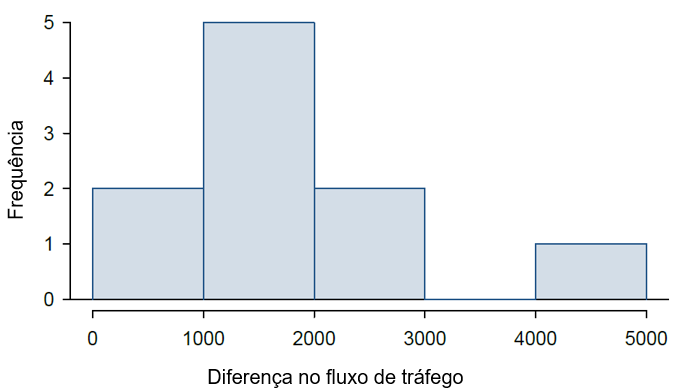
\includegraphics[width=\textwidth]{5-1_one_t/trafficHist.png}
}
\pause
\small
\justifying
\dq{Então, o que fazemos quando o tamanho da amostra é pequeno?}
\end{itemize}

$\:$ \\

\end{frame}

%%%%%%%%%%%%%%%%%%%%%%%%%%%%%%%%%%%

\begin{frame}
\frametitle{Revisão: para que serve um tamanho de amostra grande?}
\justifying
Enquanto as observações forem independentes e a distribuição da população não for extremamente assimétrica, uma grande amostra irá garantir que ...

\begin{itemize}
\justifying
\item a distribuição amostral da média é quase normal
\justifying
\item a estimativa do erro padrão, como $\frac{s}{\sqrt{n}}$, é confiável

\end{itemize}

\end{frame}

%%%%%%%%%%%%%%%%%%%%%%%%%%%%%%%%%%%

\subsection{A condição de normalidade}

%%%%%%%%%%%%%%%%%%%%%%%%%%%%%%%%%%%

\begin{frame}
\frametitle{A condição de normalidade}

\begin{itemize}
\justifying
\item O TCL, que afirma que as distribuições da amostra serão quase normais, vale para \orange{qualquer} tamanho da amostra, desde que a distribuição da população seja quase normal.

\pause
\justifying
\item Embora esse seja um caso especial bastante útil, é inerentemente difícil verificar a normalidade em conjuntos de dados pequenos.

\pause
\justifying
\item Devemos ter cautela ao verificar a condição de normalidade para amostras pequenas. É importante não só examinar os dados, mas também pensar sobre a origem dos dados.
\begin{itemize}
\justifying
\item Por exemplo, se pergunte: eu esperaria que essa distribuição fosse simétrica e estou confiante de que os outliers são raros?
\end{itemize}

\end{itemize}

\end{frame}

%%%%%%%%%%%%%%%%%%%%%%%%%%%%%%%%%%%

\subsection{Apresentando a distribuição $ t $}

%%%%%%%%%%%%%%%%%%%%%%%%%%%%%%%%%%%

\begin{frame}
\frametitle{A distribuição $ t $}

\begin{itemize}
\justifying
\item Quando o desvio padrão da população é desconhecido (o que quase sempre ocorre), a incerteza da estimativa do erro padrão é resolvida usando uma nova distribuição: a \hl{distribuição $ t $}.

\pause
\justifying
\item Essa distribuição também tem formato de sino, mas suas caudas são \hl{mais pesadas} do que as do modelo normal.

\pause
\justifying
\item Portanto, é mais provável que as observações caiam além de dois SDs da média do que sob a distribuição normal.

\pause
\justifying
\item Essas caudas mais pesadas são úteis para resolver nosso problema com uma estimativa menos confiável do erro padrão (já que $n$ é pequeno).

\end{itemize}

\begin{center}
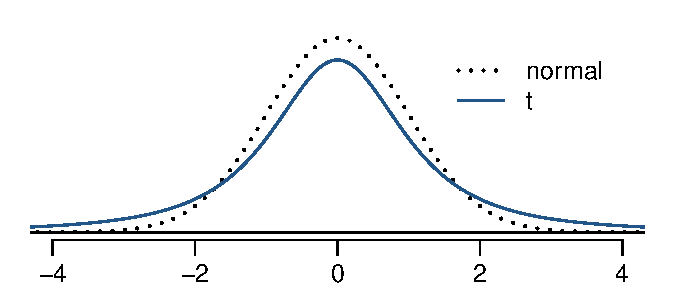
\includegraphics[width=0.4\textwidth]{5-1_one_t/tDistCompareToNormalDist.pdf}
\end{center}

\end{frame}

%%%%%%%%%%%%%%%%%%%%%%%%%%%%%%%%%%%

\begin{frame}
\frametitle{A distribuição $ t $ (cont.)}

\begin{itemize}
\justifying
\item Sempre centralizado em zero, como a distribuição normal padrão ($ z $).
\justifying
\item Tem um único parâmetro \hl{graus de liberdade}: (\mathhl{df}).

\end{itemize}

\begin{center}
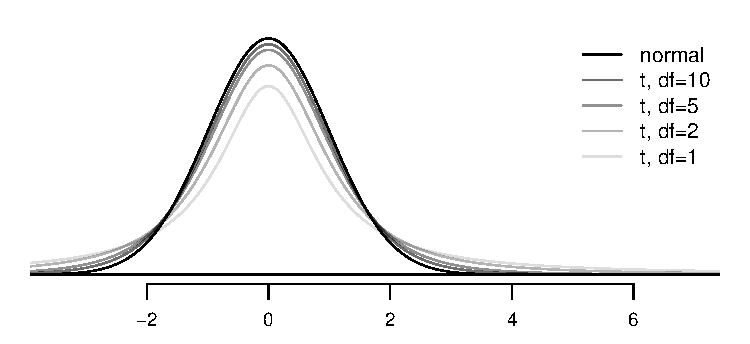
\includegraphics[width=0.8\textwidth]{5-1_one_t/tDistConvergeToNormalDist.pdf}
\end{center}

\pause
\justifying
\dq{O que acontece com a forma da distribuição $t$ quando $df$ aumenta?}
\justifying
\soln{\pause Aproxima-se da normal.}

\end{frame}

%%%%%%%%%%%%%%%%%%%%%%%%%%%%%%%%%%%

\subsection{Avaliando hipóteses usando a distribuição $t$}

%%%%%%%%%%%%%%%%%%%%%%%%%%%%%%%%%%%

\begin{frame}
\frametitle{De volta à sexta-feira 13}

{\scriptsize
\texttt{
\begin{center}
\begin{tabular}{rllrr || r || l}
  \hline
 & tipo & data & dia 6 & dia 13 & qtde & localização  \\ 
  \hline
1 & trafégo & 1990,  Julho & 139246 & 138548 & 698 & loc 1 \\
  \rowcolor[gray]{.9}
  2 & trafégo & 1990,  Julho & 134012 & 132908 & 1104 & loc 2 \\
  3 & trafégo & 1991,  Setembro & 137055 & 136018 & 1037 & loc 1 \\
  \rowcolor[gray]{.9}
  4 & trafégo & 1991,  Setembro & 133732 & 131843 & 1889 & loc 2 \\
  5 & trafégo & 1991,  Dezembro & 123552 & 121641 & 1911 & loc 1 \\
  \rowcolor[gray]{.9}
  6 & trafégo & 1991,  Dezembro & 121139 & 118723 & 2416 & loc 2 \\
  7 & trafégo & 1992,  Março & 128293 & 125532 & 2761 & loc 1 \\
  \rowcolor[gray]{.9}
  8 & trafégo & 1992,  Março & 124631 & 120249 & 4382 & loc 2 \\
  9 & trafégo & 1992,  Novembro & 124609 & 122770 & 1839 & loc 1 \\
  \rowcolor[gray]{.9}
  10 & trafégo & 1992,  Novembro & 117584 & 117263 & 321 & loc 2 \\
   \hline
\end{tabular}
\end{center}
}}
\scriptsize{
\hspace{8cm}\orange{$\downarrow$}
\begin{align*}
\hspace{6cm} &\orange{$\bar{x}_{qtde} = 1836$} \\
& \orange{$s_{qtde} = 1176$} \\
& \orange{$n = 10$} 
\end{align*}
 }
\end{frame}

%%%%%%%%%%%%%%%%%%%%%%%%%%%%%%%%%%%

\begin{frame}
\frametitle{Encontrando a estatística de teste}
\justifying
\formula{Teste estatístico: inferência para média em uma amostra pequena}
{A estatística de teste para inferência sobre a média em uma amostra pequena ($ n <50 $) é a estatística $T$ com $df = n - 1$.
\[ T_{df} = \frac{\text{esmativa pontual} - \text{valor da hipótese nula}}{SE} \]}

\pause

\vspace{-0.5cm}
\justifying
\hl{Neste contexto...}
\begin{eqnarray*}
estimativa~pontual &=& \bar{x}_{qtde} = 1836 \\
\pause
SE &=& \frac{s_{qtde}}{\sqrt{n}} = \frac{1176}{\sqrt{10}} = 372 \\
\pause
T &=& \frac{1836 - 0}{372} = 4.94 \\
\pause
df &=& 10 - 1 = 9
\end{eqnarray*}
\justifying
\scriptsize
\Note{O valor da hipótese nula é 0 porque definimos $\mu_{qtde} = 0$.}

\end{frame}

%%%%%%%%%%%%%%%%%%%%%%%%%%%%%%%%%%%

\begin{frame}[fragile]
\frametitle{Encontrando o valor p}

\begin{itemize}
\justifying
\item O valor p é, mais uma vez, calculado como sendo a área de cauda sob a distribuição $t$.

\pause

\item Usando R:
\begin{verbatim}
> 2 * pt(4.94, df = 9, lower.tail = FALSE)

[1] 0.0008022394
\end{verbatim}

\pause
\justifying
\item Usando a web app:
\justifying
\href{https://gallery.shinyapps.io/dist_calc/}{\textcolor{oiB}{https://gallery.shinyapps.io/dist\_calc/}}

\pause
\justifying
\item Se o app não estiver disponível, podemos usar uma \webLink{https://www.openintro.org/download.php?file=os2_prob_tables&referrer=/stat/textbook.php}{tabela $t$}.

\end{itemize}

\end{frame}

%%%%%%%%%%%%%%%%%%%%%%%%%%%%%%%%%%%

\begin{frame}
\frametitle{Encontrando o valor p}
\justifying
\scriptsize
Localize a estatística $ T $ calculada na linha $ df $ apropriada, obtenha o valor p do cabeçalho da coluna correspondente (uma ou duas linhas, dependendo da hipótese alternativa).

{\scriptsize
\begin{center}
\begin{tabular}{r | rrr rr}
one tail & \hspace{1.5mm}  0.100 & \hspace{1.5mm} 0.050 & \hspace{1.5mm} 0.025 & \hspace{1.5mm} 0.010 & \hspace{1.5mm} 0.005  \\
two tails & 0.200 & 0.100 & 0.050 & 0.020 & 0.010 \\
\hline
{$df$} \hfill 1  &  {  3.08} & {  6.31} & { 12.71} & { 31.82} & { 63.66}  \\ 
2  &  {  1.89} & {  2.92} & {  4.30} & {  6.96} & {  9.92}  \\ 
3  &  {  1.64} & {  2.35} & {  3.18} & {  4.54} & {  5.84}  \\ 
$\vdots$ & $\vdots$ &$\vdots$ &$\vdots$ &$\vdots$ & \\
17  &  {  1.33} & {  1.74} & {  2.11} & {  2.57} & {  2.90}  \\ 
18  &  {  1.33} & {  1.73} & {  2.10} & {  2.55} & {  2.88}  \\ 
19  &  {  1.33} & {  1.73} & {  2.09} & {  2.54} & {  2.86}  \\ 
20  &  {  1.33} & {  1.72} & {  2.09} & {  2.53} & {  2.85}  \\ 
$\vdots$ & $\vdots$ &$\vdots$ &$\vdots$ &$\vdots$ & \\
400  &  {  1.28} & {  1.65} & {  1.97} & {  2.34} & {  2.59}  \\ 
500  &  {  1.28} & {  1.65} & {  1.96} & {  2.33} & {  2.59}  \\ 
$\infty$  &  {  1.28} & {  1.64} & {  1.96} & {  2.33} & {  2.58}  \\ 
\end{tabular}
\end{center}
}
\end{frame}


\begin{frame}
\frametitle{Encontrando o valor p (cont.)}


{\scriptsize
\begin{center}
\begin{tabular}{r | rrr rr}
\hline
one tail & \hspace{1.5mm}  0.100 & \hspace{1.5mm} 0.050 & \hspace{1.5mm} 0.025 & \hspace{1.5mm} 0.010 & \hspace{1.5mm} 0.005  \\
two tails & 0.200 & 0.100 & 0.050 & 0.020 & 0.010 \\
\hline
{df} \hfill 6  &  {  1.44} & {  1.94} & {  2.45} & {  3.14} & {  3.71}  \\ 
7  &  {  1.41} & {  1.89} & {  2.36} & {  3.00} & {  3.50}  \\ 
8  &  {  1.40} & {  1.86} & {  2.31} & {  2.90} & {  3.36}  \\ 
  \rowcolor[gray]{.6}
9  &  {  1.38} & {  1.83} & {  2.26} & {  2.82} & {  3.25}  \\ 
10  &  {  1.37} & {  1.81} & {  2.23} & {  2.76} & {  3.17}  \\ 
\end{tabular}
\vspace{1cm}
\twocol{0.5}{0.5}{
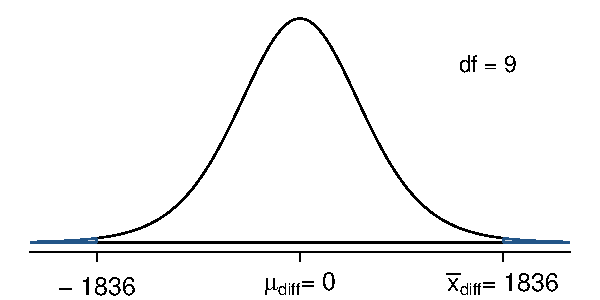
\includegraphics[width=1.1\textwidth]{5-1_one_t/fridayPvalue.pdf}
}
{
$T = 4.94$}

\end{center}
}

\end{frame}

%%%%%%%%%%%%%%%%%%%%%%%%%%%%%%%%%%%

\begin{frame}
\frametitle{Conclusão do teste}
\justifying
\dq{Qual é a conclusão do teste de hipóteses?}
\justifying
\pause
\soln{Os dados fornecem evidências convincentes de uma diferença entre o fluxo de tráfego na sexta-feira 6 e 13.}


\end{frame}

%%%%%%%%%%%%%%%%%%%%%%%%%%%%%%%%%%%%

\subsection{Construindo intervalos de confiança usando a distribuição $t$}

%%%%%%%%%%%%%%%%%%%%%%%%%%%%%%%%%%%

\begin{frame}
\frametitle{Qual é a diferença?}

\begin{itemize}
\justifying
\item Concluímos que há uma diferença no fluxo de tráfego entre sexta-feira 6 e 13.

\pause
\justifying
\item Mas seria mais interessante descobrir exatamente que diferença é essa.

\pause
\justifying
\item Podemos usar um intervalo de confiança para estimar essa diferença.

\end{itemize}

\end{frame}

%%%%%%%%%%%%%%%%%%%%%%%%%%%%%%%%%%%

\begin{frame}
\frametitle{Intervalo de confiança para uma média em uma amostra pequena}

\begin{itemize}
\justifying
\item Os intervalos de confiança são sempre da forma
\[ \text{estimativa pontual} \pm {ME} \]

\pause
\justifying
\item ME é sempre calculado como o produto entre o valor crítico e o SE.

\pause
\justifying
\item Uma vez que uma amostra pequena significa uma distribuição de $t$ (e não uma distribuição de $z$), o valor crítico é $t^{\star}$ (ao contrário de $z^{\star}$).
\[ \text{estimativa pontual} \pm t^{\star} \times SE \]

\end{itemize}

\end{frame}

%%%%%%%%%%%%%%%%%%%%%%%%%%%%%%%%%%%

\begin{frame}
\frametitle{Encontrando o valor crítico $t$ ($t^\star$)}

\twocol{0.5}{0.5}{
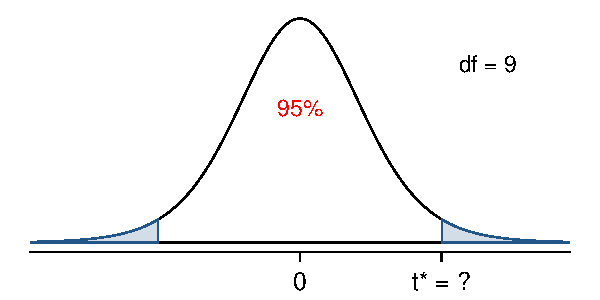
\includegraphics[width=\textwidth]{5-1_one_t/middle95_1.pdf}
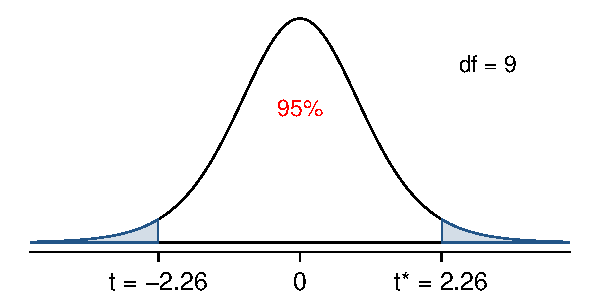
\includegraphics[width=\textwidth]{5-1_one_t/middle95_2.pdf}
}
{\justifying
$n = 10$, $df = 10 - 1 = 9$, $t^\star$ está na interseção da linha $ df = 9 $ e duas probabilidades da cauda 0.05.
}

\end{frame}
%%%%%%%%%%%%%%%%%%%%%%%%%%%%%%%%%%%

\begin{frame}
\frametitle{Encontrando o crítico $t$ ($t^\star$)}
\only<1>{
{\small
\begin{center}
\begin{tabular}{r | r r r r r}
\hline
Uma cauda & \hspace{1.5mm}  0.100 & \hspace{1.5mm} 0.050 & \hspace{1.5mm} 0.025 & \hspace{1.5mm} 0.010 & \hspace{1.5mm} 0.005  \\
duas caudas & 0.200 & 0.100 & 0.050 & 0.020 & {0.010} \\
\hline
{df} \hfill 6  &  {  1.44} & {  1.94} & {  2.45} & {  3.14} & {  3.71}  \\ 
7  &  {  1.41} & {  1.89} & {  2.36} & {  3.00} & {  3.50}  \\ 
8  &  {  1.40} & {  1.86} & {  2.31} & {  2.90} & {  3.36}  \\ 
9  &  {  1.38} & {  1.83} & {  2.26} & {  2.82} & {  3.25} \\ 
10  &  {  1.37} & {  1.81} & {  2.23} & {  2.76} & {  3.17}  \\ 
\end{tabular}
\end{center}
}}

\only<2 | handout:0>{
{\small
\begin{center}
\begin{tabular}{r | r r r r r}
\hline
Uma cauda & \hspace{1.5mm}  0.100 & \hspace{1.5mm} 0.050 & \hspace{1.5mm} 0.025 & \hspace{1.5mm} 0.010 & \hspace{1.5mm} 0.005  \\
duas caudas & 0.200 & 0.100 & 0.050 & 0.020 & {0.010} \\
\hline
{df} \hfill 6  &  {  1.44} & {  1.94} & {  2.45} & {  3.14} & {  3.71}  \\ 
7  &  {  1.41} & {  1.89} & {  2.36} & {  3.00} & {  3.50}  \\ 
8  &  {  1.40} & {  1.86} & {  2.31} & {  2.90} & {  3.36}  \\ 
  \rowcolor[gray]{.6}
9  &  {  1.38} & {  1.83} & {  2.26} & {  2.82} & {  3.25} \\ 
10  &  {  1.37} & {  1.81} & {  2.23} & {  2.76} & {  3.17}  \\ 
\end{tabular}
\end{center}
}}

\only<3 | handout:0>{
{\small
\begin{center}
\begin{tabular}{r | r r >{\columncolor[gray]{.6}[.5\tabcolsep]}r r r}
\hline
Uma cauda & \hspace{1.5mm}  0.100 & \hspace{1.5mm} 0.050 & \hspace{1.5mm} 0.025 & \hspace{1.5mm} 0.010 & \hspace{1.5mm} 0.005  \\
duas caudas & 0.200 & 0.100 & \orange{0.050} & 0.020 & {0.010} \\
\hline
{df} \hfill 6  &  {  1.44} & {  1.94} & {  2.45} & {  3.14} & {  3.71}  \\ 
7  &  {  1.41} & {  1.89} & {  2.36} & {  3.00} & {  3.50}  \\ 
8  &  {  1.40} & {  1.86} & {  2.31} & {  2.90} & {  3.36}  \\ 
  \rowcolor[gray]{.6}
9  &  {  1.38} & {  1.83} & {  2.26} & {  2.82} & {  3.25} \\ 
10  &  {  1.37} & {  1.81} & {  2.23} & {  2.76} & {  3.17}  \\ 
\end{tabular}
\end{center}
}}

\only<4 | handout:0>{
{\small
\begin{center}
\begin{tabular}{r | r r >{\columncolor[gray]{.6}[.5\tabcolsep]}r r r}
\hline
Uma cauda & \hspace{1.5mm}  0.100 & \hspace{1.5mm} 0.050 & \hspace{1.5mm} 0.025 & \hspace{1.5mm} 0.010 & \hspace{1.5mm} 0.005  \\
duas caudas & 0.200 & 0.100 & \orange{0.050} & 0.020 & {0.010} \\
\hline
{df} \hfill 6  &  {  1.44} & {  1.94} & {  2.45} & {  3.14} & {  3.71}  \\ 
7  &  {  1.41} & {  1.89} & {  2.36} & {  3.00} & {  3.50}  \\ 
8  &  {  1.40} & {  1.86} & {  2.31} & {  2.90} & {  3.36}  \\ 
  \rowcolor[gray]{.6}
9  &  {  1.38} & {  1.83} & \orange{  2.26} & {  2.82} & {  3.25} \\ 
10  &  {  1.37} & {  1.81} & {  2.23} & {  2.76} & {  3.17}  \\ 
\end{tabular}
\end{center}
}}


\end{frame}

%%%%%%%%%%%%%%%%%%%%%%%%%%%%%%%%%%%

\begin{frame}
\frametitle{Construindo um IC para uma média pequena de amostra}
\justifying
\pq{Qual dos seguintes é o cálculo correto de um intervalo de confiança de 95\% para a diferença entre o fluxo de tráfego entre sexta-feira 6 e 13?}
\[ \bar{x}_{qtde} = 1836 \qquad s_{qtde} = 1176 \qquad n = 10 \qquad SE = 372 \]

\twocol{0.35}{0.65}
{
\begin{enumerate}[(a)]

\item $1836 \pm 1.96 \times 372$

\solnMult{ $1836 \pm 2.26 \times 372$}

\item $1836 \pm -2.26 \times 372$

\item $1836 \pm 2.26 \times 1176$

\end{enumerate}
}
{
\soln{\only<2>{\orange{$\rightarrow$ (995, 2677)}}}
\vspace{0.25cm}
}

\end{frame}

%%%%%%%%%%%%%%%%%%%%%%%%%%%%%%%%%%%

\begin{frame}
\frametitle{Interpretando o IC}
\justifying
\pq{Qual das seguintes opções é a \orange{melhor} interpretação para o intervalo de confiança que acabamos de calcular?
\[ \mu_{qtde: 6 - 13} = (995, 2677) \]
}
\justifying
Estamos 95\% confiantes de que ...

\begin{enumerate}[(a)]
\justifying
\item a diferença entre o número médio de carros na estrada na sexta-feira 6 e 13 é entre 995 e 2.677.
\justifying
\item na sexta-feira 6 há 995 a 2.677 carros a menos na estrada do que na sexta-feira 13, em média.
\justifying
\item na sexta-feira 6 há, em média, 995 carros a menos e na sexta-feira 13 há, em média, 2.677 carros a mais na estrada.
\justifying
\solnMult{na sexta-feira 13 há de 995 a 2.677 carros a menos na estrada do que na sexta-feira 6, em média.}

\end{enumerate}

\end{frame}

%%%%%%%%%%%%%%%%%%%%%%%%%%%%%%%%%%%

\subsection{Síntese}

%%%%%%%%%%%%%%%%%%%%%%%%%%%%%%%%%%%

\begin{frame}
\frametitle{Síntese}
\justifying
\dq{A conclusão do teste de hipótese concorda com o que encontramos para o intervalo de confiança?}

$\:$ \\
\justifying
\soln{\only<2->{Sim, o teste de hipótese encontrou uma diferença significativa e o IC não contém o valor da hipótese nula que é igual zero.}}

$\:$ \\
\justifying
\dq{Você acha que as descobertas deste estudo sugerem que as pessoas acreditam que sexta-feira 13 é um dia de má sorte?}

$\:$ \\
\justifying
\soln{\only<3>{Não, este é um estudo observacional. Acabamos de observar uma diferença significativa entre o número de carros na estrada nesses dois dias. Nós não testamos as crenças das pessoas.}}

\end{frame}

%%%%%%%%%%%%%%%%%%%%%%%%%%%%%%%%%%%

\begin{frame}

\frametitle{Recapitulando: Inferência usando a distribuição $t$}

\begin{itemize}

\justifying
\item Se $ \sigma $ for desconhecido, use a distribuição $t$ com $SE = \frac{s}{\sqrt {n}}$.

\pause
\justifying
\item Condições: 
\begin{itemize}
\justifying
\item independência das observações (usar amostragem aleatória, e se a amostragem for sem reposição, $n <$ 10\% da população)
\justifying
\item nenhum desvio extremo
\end{itemize}

\end{itemize}

\end{frame}

\begin{frame}

\frametitle{Recapitulando: Inferência usando a distribuição $t$}

\begin{itemize}
\justifying

\item Teste de hipóteses: 
\[ T_{df} = \frac{\text{estimativa pontual} - \text{valor da hipótese nula}}{SE}\text{, onde }df = n - 1 \]

\pause
\justifying
\item Intervalo de confiança:
\[ \text{estimativa pontual} \pm t_{df}^\star \times SE \]

\end{itemize}

\pause
\Note{\scriptsize O exemplo que usamos foi para médias pareadas (diferença entre grupos dependentes). Tomamos a diferença entre as observações e usamos apenas essas diferenças (uma amostra) em nossa análise, portanto, a mecânica é a mesma de quando estamos trabalhando com apenas uma amostra.}
\end{frame}
